\documentclass[11pt]{article}
\usepackage{/Users/mz/Box/repository/LaTeX/article}
\title{Do Mass Shootings Influence Change in American's Support for Gun Control? A Replication and Extension of Rogowski and Tucker (2019)}
\author{Name Redacted}
\date{\today}
\bibliography{ref}

\begin{document}

\maketitle

\section*{Introduction}
Are critical public events able to influence attitude change, or do these events fail to galvanise widespread support? On the 1\textsuperscript{st} May, 2020, Justin Trudeau introduced new legislation to ban assault weapons following Canada’s worst mass shooting in history. Research conducted by the Angus Reid Institute suggests that 65\% of a nationally representative sample of Canadians support the complete ban of civilians possessing assault-style weapons \autocite{angus-reid-institute2020four-in-five-ca}. These sentiments are echoed by a strand of literature in the field of public opinion, which suggests that significant events can motivate attitude change by bringing the events focus into the public realm \autocites{carmines1989issue-evolution}{zaller1992the-nature-and-}. This topic is central to the article by \textcite[][the two authors are hereafter abbreviated as RT]{rogowski2019critical-events}, titled ``Critical events and attitude chang'', which attempts to explore support for gun control after a mass shooting. Particular emphasis is placed on whether attitudes towards gun control changed following the Sandy Hook Elementary School shooting in Newtown, Connecticut, which resulted in the death of 26 people, many of whom were children. The authors leveraged the staggered timing of the survey which saw the shooting fell between waves 12 and 13 of The American Panel Survey (TAPS), in order to gauge whether public opinion towards gun control changed as a result of this event. Their analysis highlights that following the occurrence of a significant public event, support for gun control did not increase. What is more, the attitudes of Americans towards gun control are deeply entrenched and unmalleable to critical events such as mass shootings.

In light of these conclusions, the current study aims to replicate RT’s findings and then extend them further. Several recent studies have reported contradictory findings to those noted by RT \autocites{wozniak2015american-public}{newman2019mass-shootings-}{barney2019reexamining-the}. This therefore serves as sufficient evidence to assess the robustness of their claims through a re-examination of their data. In the extension element of our replication project, we firstly add in an important co-variate which we believe should be included in the analysis, education. Following this, we also test the robustness of RT's conclusions on a separate wave of TAPS to further explore the validity of their findings. Specifically, we use TAPS wave 55 occurred in June 2016, which is situated around the time of the Orlando shooting which resulted in 49 dead and a further 53 wounded. Given that the magnitude (i.e., the death count), and situational timing of the Orlando and Sandy Hook School shootings are similar, we believe that comparisons can be drawn between the two. 

On this premise, we will first provide a brief overview of recent research in this field. A general outline of attitudes towards gun control will be provided, noting recent polling evidence. This will be followed by a section detailing recent experimental research using exogenous events. The scholarly literature in this field has recently been mired by a number of claims both supporting and refuting calls for increased gun control. Next, we will then report our attempt at replicating the findings of RT. From our analysis, we note that the conclusions drawn by the authors are replicable and robust. Following on, we will aim to extend these analyses by testing two additional hypotheses. The first, is the addition of an important co-variant not previously included by the authors. Thus, we include education into our analysis to examine whether the Sandy Hook shooting's effect on gun control support is present conditional on one's educational level. In such case, the results are null and no change in attitudes towards gun control are observed. The second hypothesis extends the analysis to a separate data set of TAPS, wave 55, following June 2016 Orlando shooting. This was done to explore whether the null results reported by RT were a product of the question used to quantify attitude change. A separate data set was used that employs a broader set of gun control questions. Here, we further demonstrate that the null results hold true; attitudes towards gun control are deeply entrenched and fail to be influenced by mass shootings.

\section*{Attitudes towards Gun Control}
The ongoing debate around gun control in the US has intensified over the past decade. Several high-profile mass shootings have received wide-spread coverage that has seen bipartisan condemnation. Whilst opinion polls suggest a slight increase in the general public’s support for gun control, the picture is not clear cut. Longitudinal research conducted by the Pew Research Centre between 1993 and 2019 highlights that support has varied over the years, ranging from 66\% who support increased gun control in March 2000, to a low of 46\% in December 2014 \autocite{schaeffer2019share-of-americ}. Despite this, support for tighter gun control laws has seen a slight increase overall. With that being said, gun control is a broad topic and some areas have received greater support than others. For example, Americans have become more in favour of banning high-capacity ammunition magazines, with 71\% favouring a ban in 2019 compared to 65\% in 2017. Moreover, appetite has also increased for greater background checks, the banning of assault style weapons, and preventing those with mental illnesses from purchasing guns \autocite{schaeffer2019share-of-americ}. The multifaceted nature of the gun control debate becomes even more convoluted when factoring in who supports or opposes these changes. Polling data suggests that the American public does not have a homogenous view when it comes to their attitudes towards gun control. The greatest disparity in attitudes derives from partisan affiliation, with 65\% of Democrats who favour increased gun control in 2014 compared to 75\% of Republicans who believe that the rights of Americans to own guns should be protected \autocite{doherty2015a-public-opinio}.

Other demographics are also highly correlated with attitudes towards gun control. Women, for example, are more likely to favour stricter gun laws with 64\% in support, compared to 55\% of men \autocite{schaeffer2019share-of-americ}. Those who have studied at university are also more likely to support such measures than those who have not. These differentiating characteristics are highlighted by \textcite{smith2002public-opinion-}, who notes that ``Women, residents of large cities and their suburbs, liberals, and Democrats are most likely to support general gun control measures, whereas, men, residents of rural areas, conservatives, and Republicans are least likely to support such measures''. As such, this demonstrates that the debate around gun control does not only revolve around a specific topic or policy, but attitudes may also differ between different strata of society.

\section*{Experimental Research}
Although there are notable differences highlighted by opinion polls between gun control advocates and those who oppose such restrictions, experimental evidence has been less conclusive. This type of experimental research usually functions through measuring the change in opinion as a direct result of an exogenous event, such as a mass shooting. Recent studies have further highlighted the complexity of this debate. For example, research conducted by \textcite{newman2019mass-shootings-} has explored the role of geographical proximity to mass shooting events and whether this affects attitude change towards gun control. Data was analysed from multiple sources, including the 2010 Cooperative Congressional Election Study (CCES), which is a panel survey that allowed for the assessment of attitudes towards mass shooting events between 1996 and 2015. Participant’s geographical locations were geotagged using zip codes to establish whether preferences for gun control were associated with closer proximity to a mass shooting. All in all, 210 mass shooting events were identified and all those who fell within a 100 mile distance were classified as ‘proximate’, whilst those who fell outside of this range were deemed as ‘distal’. The results suggest that those who are geographically proximate to a mass shooting event are more likely to support stricter gun control regulations. Those who live within a 100 mile distance of a shooting event are on average more likely to support increases in general gun controls. What is more, the authors note that this effect does not vary with partisanship, with republicans and democrats holding the same valence towards gun control, whether they are deemed proximate or distant. In such cases, partisans possess the same directionality of attitudes in either condition, with both groups being more (or less) in support based on whether they are closer (or further) for the shooting event. Democrats were more in favour of tighter gun controls and Republicans were less in favour of gun control, irregardless of their proximity.

In a follow-up study, \textcite{barney2019reexamining-the} attempted to replicate the findings of Newman and Hartman and extend them further. Using a methodology that was identical to the original study, Barney and Schaffner found various discrepancies between their analysis and the conclusions highlighted by Newman and Hartman. Crucially, they identified that participant’s proximity was incorrectly coded, resulting in erroneous counts in the number of participants who  resided within the 100 mile radius. When this mistake was corrected for, the proximity of those close to mass shooting events did not influence a change in gun control attitudes. This effect also failed to emerge when altering the distance of those determined as ‘proximate’ to varying distances from the shooting event (i.e., \(<\) 10, \(<\) 25, \(<\) 50, \(<\) 100 miles). However, Barney and Schaffner report that proximity does have a polarising effect when taking into account partisanship. Democrats become more strongly in favour of gun control the closer they are to a mass shooting, whilst Republicans become more opposed to such restrictions. In sum, these findings suggest that the proximity to a mass shooting does not influence support for increased gun controls, but does influence attitudinal polarisation based on partisan differences. The result of which is that both republicans and democrats views became more entrenched. 

Why are these results important? The rational for this is twofold. Firstly, these findings further demonstrate the complex and precarious nature of attitudes towards gun control. They illustrate that gun control attitudes are not a unidimensional construct and crucially depend on a number of different elements. So far, a number of significant factors have been highlighted in the context of experimental research, including partisanship and geographical proximity. In our extension of RT's study, we also aim to incorporate educational attainment into the analysis. This will allow us to further explore which factors are influential in this process. Second, given that Barney and Schaffner provide evidence of a failed replication attempt in this field, this also serves to strengthen the justification for our replication. 

\section*{Replication}
\subsection*{Procedural Replication}
RT used the staggered nature of survey questionnaire waves to evaluate the causal effect of the Sandy Hook shooting, which happened on the December 14\textsuperscript{th} 2012, on American people’s gun control attitude. Since the shooting timing is convincingly exogenous, are assigned in a quasi random fashion to pre- and post-shooting groups. Crucially, this is according to whether they completed the questionnaire before or after the 14\textsuperscript{th} of December. The pre-shooting group is therefore the control group and the post-shooting group receives the treatment | the exposure to the tragic mass shooting. In principle, this quasi random assignment holds a number of key variables constant with regards to their attitudes towards gun control. The exception to this is the recent exposure to the Sandy Hook School shooting. Thus, any detected difference in gun control attitudes among survey respondents may be attributed to the shooting event.\footnote{See \textcite{munoz2020unexpected-even} for a detailed discussion on further assumptions needed to make a valid causal inference using this sort of research design.}

The data source used by RT is TAPS, which is a longitudinal (on a monthly basis), internet-based public opinion survey targeted towards a national representative sample of US adults. The survey employs an adjusted weight that enables the data to be more representative of the US adult population. RT used wave 13 (December 2012) alone for the cross-sectional analysis:
\begin{align}
y_{i} = \alpha + \beta t_{i} + \epsilon_{i},\label{eq1}
\end{align}
in which \(y_i\) denotes the respondent \(i\)’s gun control attitude, \(t_i = 0, 1\) indicates the treatment (exposure to the Sandy Hook shooting or not), and \(\beta\) is the treatment effect. RT also used wave 13 and 14 (January 2013) for the panel analysis. In this sample, only the respondents who finished the wave 13 survey before the Sandy Hook shooting are kept. The analysis actually is a within-respondent estimation:
\begin{align}
\Delta y_{i} = \alpha + \epsilon_{i},\label{eq2}
\end{align}
in which \(\Delta y_{i} = y_{i}^{\text{Jan}} - y_{i}^{\text{Dec}}\), and \(\alpha\) is the treatment effect. 

RT measured the dependent variable, gun control attitude, through the following question (the code for this question in TAPS’ official data manual and datasets are \texttt{IGUNS13} (wave 13) and \texttt{IGUNS14} (wave 14)):
\begin{displayquote}
\itshape
Federal law should ban the possession of handguns except by law enforcement personnel. Indicate your level of agreement with this statement.
\end{displayquote}
All responses were plotted along a 5-point Likert scale, where 1 = Strongly Disagree, 3 = Neither Disagree nor Agree, and 5 = Strongly Agree.\footnote{In the original dataset, 1 meant strongly agree while 5 meant the opposite. We have reversed this order to make it more intuitive.} Only 8 and 5 respondents refused to give an answer to this question in wave 12 and 13 respectively so these observations were removed from the analysis.

It could be the case that the Sandy Hook shooting’s effect is heterogenous among different groups of people. If all respondents are simply pooled together, the bi-directional effects are likely to off-set each other, resulting an overall null finding. Hence, RT run a series of sub-sample analyses to see whether attitudes change for a particular group. The group indicators are party affiliation (Democrats, Republicans, Independents), ideology (liberal, moderate, conservative), gender, parental status, the National Rifle Association (NRA) membership, and the geographical proximity to Newtown, Connecticut, where the shooting happened.  

In RT’s main analysis, the 5-point dependent variable is collapsed to a dichotomous response. They treated 'Agree' and 'Strongly Agree' as support for increased gun control (coded as 1), while all other responses were coded as not support (coded as 0). In the appendix, the ordinal version is used. Through the analysis, they treated the dependent variable as a continuous one and therefore used the least squares (LS) estimation. RT applied the survey weight for all analyses to make findings more applicable to the general US adult population.

After exactly following all the procedures RT employed, we are able to identically replicate the numerical results reported by them.\footnote{RT showed the results via coefficient plots. For the underlying numbers, see the Stata log file in RT’s Harvard Dataverse repository. Between RT’s results and ours, there are negligible 0.001-difference in some reported uncertainty estimates (standard errors, \(t\)-statistics, and \(p\)-values). We believe this is because RT used Stata while we use R and there are some minor discrepancy in terms of the rounding procedure between them when reporting result. And since Stata is proprietary while R is open-source, their computational routines could be slightly different after the computation becomes complicated. According to our experience, for instance, Stata and R oftentimes produce minor differences when clustered standard errors are used.} Specifically, in the cross-sectional analyses, no matter the dependent variable is binary (\hyperref[atab1]{Table 3 in Appendix}) or ordinal (\hyperref[atab2]{Table 4 in Appendix}), none \(p-\)values are below the \(\alpha = 0.05\) threshold, implying we do not have sufficient statistical evidence to reject the null hypothesis | the Sandy Hook shooting does not alter American people’s gun control attitude. In the panel analyses, there are few statistically significant results, but strikingly, the estimated signs are against what conventional wisdom suggests. For instance, respondents who self-identified as liberal are 8.2\% less likely to support gun control after being exposed to the Sandy Hook shooting (\(p = 0.002\), see \hyperref[atab3]{Table 5 in Appendix}). When the ordinal dependant variable is used (\hyperref[atab4]{Table 6 in Appendix}), the effect for liberal people is \(-0.147\) (\(p = 0.035\)), meaning that for liberal people, the exposure to the Sandy Hook shooting linearly decreases their support of gun control by 0.15 in a 5-points scale. These effects mean the Sandy Hook shooting, which took 20 children’s life away tradgically, even decreased the gun control support of those whose predisposition is gun control-favoured.

\subsection*{Robustness Replication}
Do the overall null findings reported by RT reflect of the populations attitudes towards gun control? In this part, we check the robustness of RT's results. Although the dependent variable is categorical in nature, RT treat it as a continuous variable and use LS estimation throughout their analyses (in both the main text and appendix). We fully acknowledge that (a) the coefficient equals the quantity of interest in LS so when the dependent variable is categorical, the LS results are easier-to-interpret; (b) LS could be more computationally robust than maximum likelihood (ML); and (c) LS produces substantively indifferent results compared to other models in many empirical cases and it is a workhorse, or even default, model in some fields. However, at least in the current political science profession, it is nearly an industry-standard that when LS is used for the categorical variable, a generalized linear model (GLM) estimated by ML should be applied for the robustness checks (and \emph{vice versa}). Since RT failed to follow this convention, we use logit model (\hyperref[eq3]{Equation 3}) and ordered logit model (\hyperref[eq4]{Equation 4}) to re-estimate the binary dependent variable and ordinal dependent variable respectively:
\begin{align}
\ln\frac{\text{Pr}(y_i = 1)}{1 - \text{Pr}(y_i = 1)} & = \alpha + \beta t_{i},\label{eq3}\\
\ln\frac{\text{Pr}(y_i \leq j|t_i)}{\text{Pr}(y_i \geq j|t_i)} & = \tau_{j|j+1} - \beta t_i,\label{eq4}
\end{align}
in which \(\beta t_i\) is defined as same as that in \hyperref[eq1]{Equation (1)}. In \hyperref[eq4]{Equation (4)}, \(j\) denotes the ordered categories from strongly disagree (coded as 1) to agree (coded as 4) and \(\tau_{j|j+1}\) is cut point.\footnote{\(\text{Pr}(y_i \leq \text{strongly agree (coded as 5)}|t_i) = 1\), which is trivial. So \(j = 1, 2, 3, 4.\)}

Since all estimates from RT’s cross-sectional design are statistically insignificant, we focus on only the cross-sectional sample (i.e., wave 13) only to see whether these counter-intuitively null results are robust under the alternative estimation frameworks. In addition, we only reassess the cross-sectional sample due to compliance concerns. Whether the treatment group subjects comply with the assigned treatment is an issue in any kinds of experimental studies. In RT’s research setting, non-compliance happens if a post-shooting respondent has not enough cognitive exposure to the shooting itself. Since all respondents in the panel sample answered the post-shooting survey questionnaire about one month later, whether the Sandy Hook tragedy is still present in their cognitive activities at that time is doubtful. In other words, the panel sample respondents are more likely to be less compliant with the treatment. In contrast, the gap between the shooting and survey completion day in the cross-sectional sample is much shorter, meaning that the respondents are more likely to comply. We discard all survey weight from our analyses in this part to have less conservative uncertainty estimates, which are more likely to lead to statistically significant results. Our logic is if the reported null results from RT remained unchanged even under a statistical significance-favoured condition, the null results are robust.

After running the logit model, we use \(\displaystyle{\widehat{{\text{Pr}(y_i = 1)}} = \frac{\exp(\hat{\alpha} + \hat{\beta} t_{i})}{1 + \exp(\hat{\alpha} + \hat{\beta} t_{i})}}\) to calculate the predicted probability of gun control support when \(t_i = 0\) (pre-shooting) and \(t_i = 1\) (post-shooting) and visually show them in \hyperref[fig1]{Figure 1}. The over-lapping of all confidence intervals indicate that \(\widehat{\text{Pr}(y_i = 1|t = 0)}\) is not statistically different from \(\widehat{\text{Pr}(y_i = 1|t = 1)}\). Substantively, it suggests we do not have sufficient evidence to claim the Sandy Hook shooting change American people’s gun control attitude, regardless of their group characteristics. Our logit model results perfectly corroborate the null finding in RT.

Our results change slightly when the ordered logit model is applied. In \hyperref[tab1]{Table 1}, the exponentiated estimated coefficients quantify the odds (\(\frac{p}{1-p}\)) ratio of moving from a lower category (less supportive of gun control) to a higher category (more supportive of gun control) between the pre-shooting and post-shooting groups. A greater-than-one quantity means an increase in odds, and therefore, demonstrates a positive effect of the Sandy Hook shooting on support for gun control. The \(p\)-values associated with Republicans and Conservative are both below the \(\alpha = 0.05\) threshold, indicating the Sandy Hook shooting’s statistically significant effect on these two groups. Surprisingly, the exponentiated estimates for these two groups are both greater than one. This result suggests although the Sandy Hook shooting does not change most American people’s gun control attitude, it made Republicans and Conservatives more supportive of gun control. In general, these groups are typically opposed to tighter gun controls and these findings are on the contradict this. More specifically, the Sandy Hook School shooting increases the odds of upward gun control attitudes by 50\%. Overall, under the different estimation frameworks and a significance-favoured condition (estimation without the survey weight), we find the null finding in RT still largely holds.
\begin{figure}[htbp!]
\centering
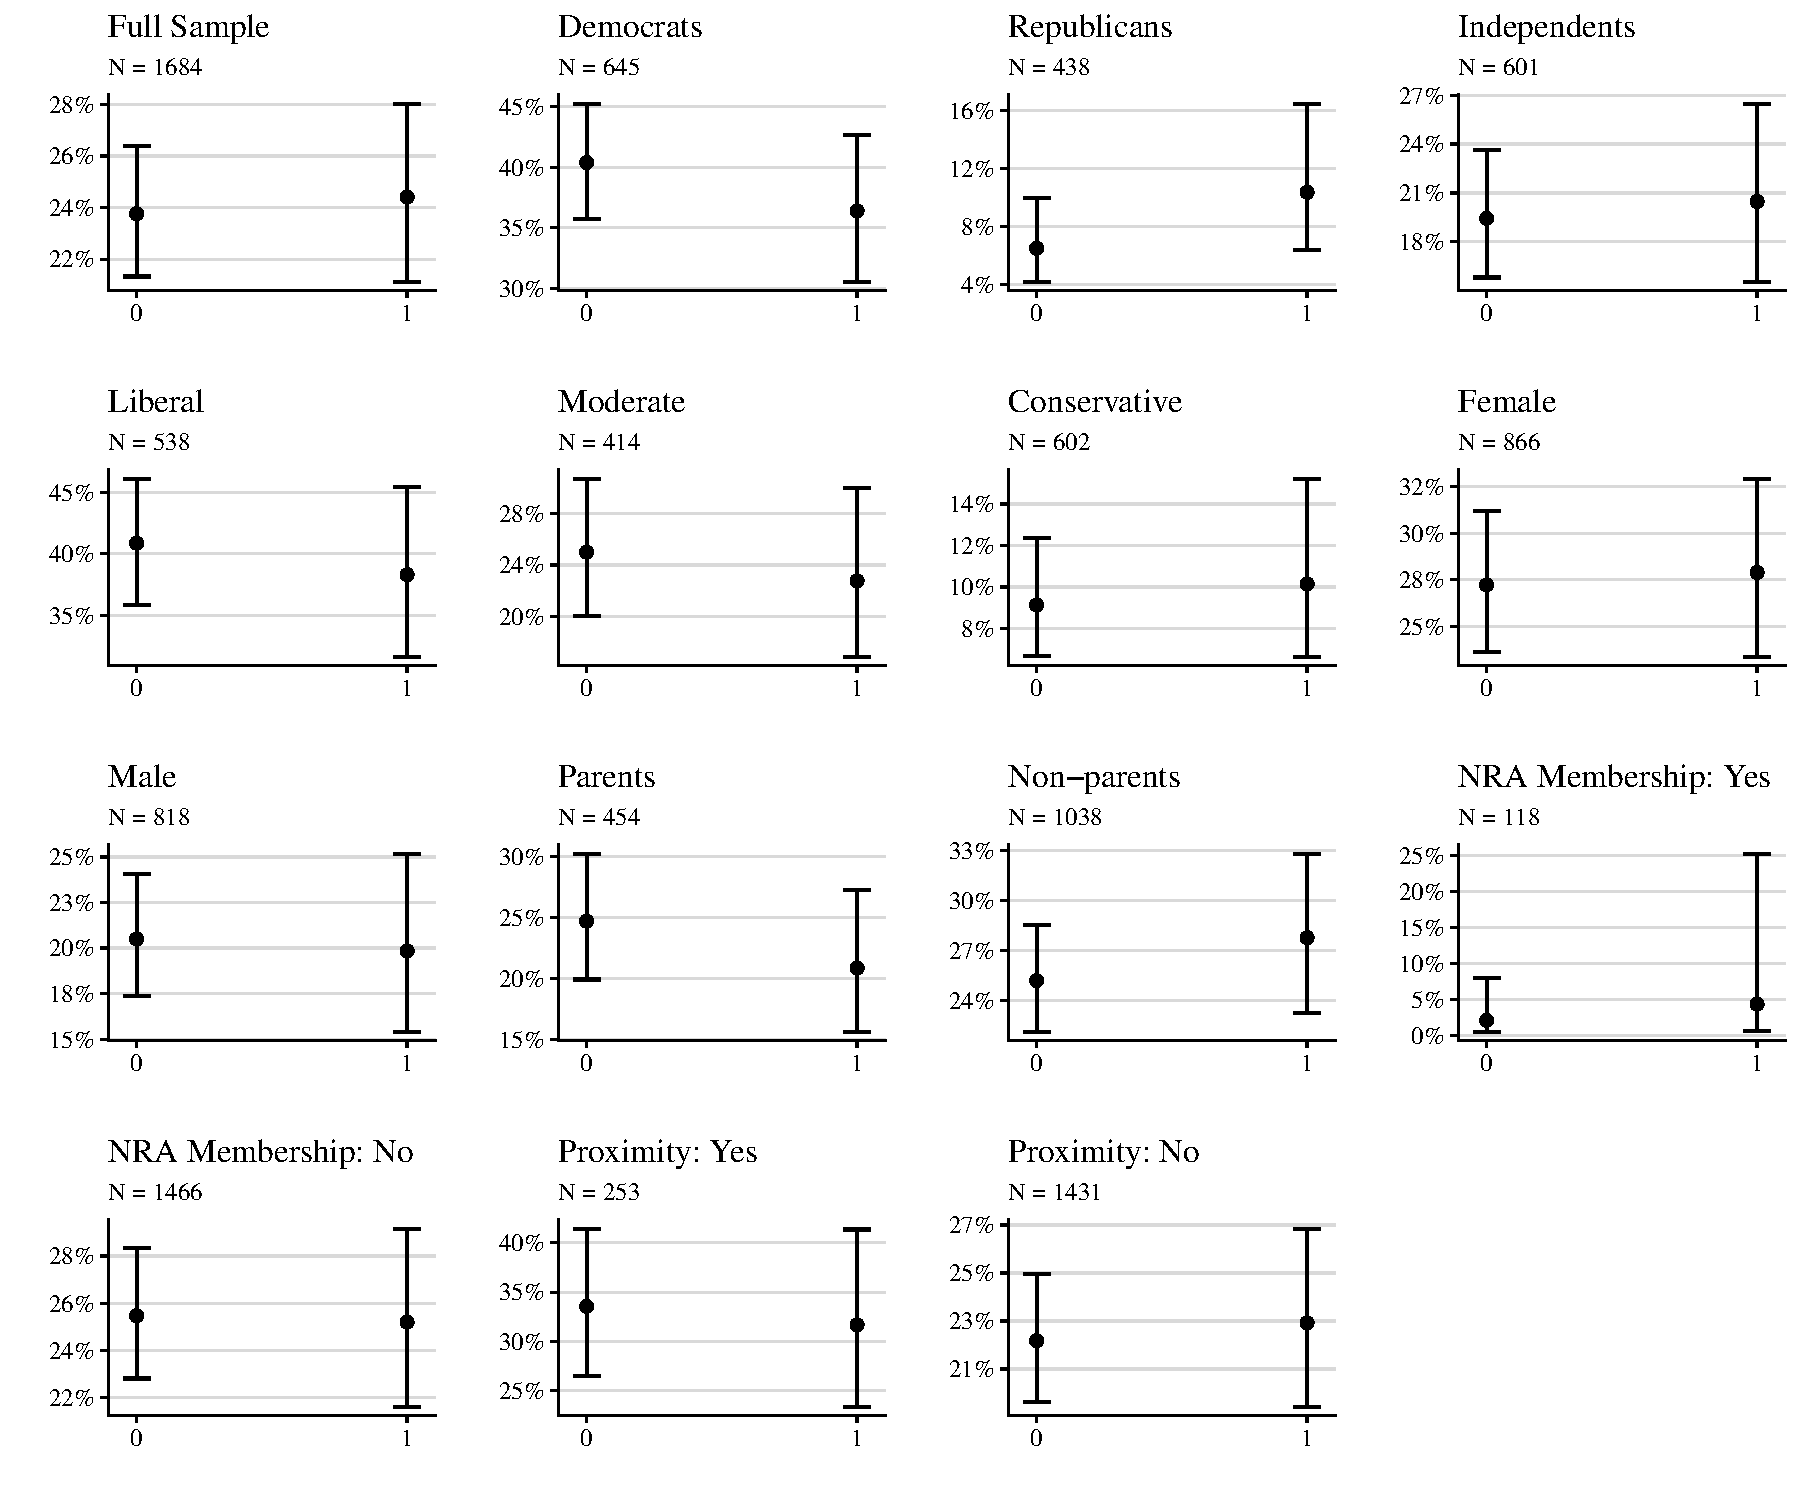
\includegraphics[width = 0.9\linewidth]{/Users/mz/Box/repository/replication/rogowski_tucker_2019_psrm/figs/fig1.pdf}
\captionsetup{justification = raggedright, singlelinecheck = false}
\caption{Predicted probabilities of gun control support (support = 1) before and after the 2012 Sandy Hook shooting. In the \(x\)-axis, 0 means pre-shooting and 1 means post-shooting. The error bars show the 95\% confidence interval, which are calculated by the Delta method.}\label{fig1}
\end{figure}
% latex table generated in R 4.0.0 by xtable 1.8-4 package
% Wed May 13 22:27:16 2020
\begin{table}[ht]
\centering
\caption{Effect of the Sandy Hook Shooting on Gun Control Support (5-points Likert Scale), Ordered Logit Results} 
\label{tab1}
\begin{tabular}{lccrrr}
  \toprule
 & Estimate & Standard Error & \(z\)-statistic & \(p\)-value & \(N\) \\ 
  \midrule
Full Sample & 1.144 & 0.091 & 1.475 & 0.140 & 1684 \\ 
  Democrats & 0.892 & 0.145 & $-$0.788 & 0.431 & 645 \\ 
  Republicans & 1.524 & 0.200 & 2.109 & 0.035 & 438 \\ 
  Independents & 1.169 & 0.154 & 1.013 & 0.311 & 601 \\ 
  Liberal & 0.923 & 0.161 & $-$0.496 & 0.620 & 538 \\ 
  Moderate & 1.002 & 0.180 & 0.010 & 0.992 & 414 \\ 
  Conservative & 1.495 & 0.168 & 2.388 & 0.017 & 602 \\ 
  Female & 1.036 & 0.124 & 0.287 & 0.774 & 866 \\ 
  Male & 1.174 & 0.137 & 1.169 & 0.242 & 818 \\ 
  Parents & 1.019 & 0.170 & 0.110 & 0.912 & 454 \\ 
  Non-parents & 1.148 & 0.119 & 1.160 & 0.246 & 1038 \\ 
  NRA Membership: Yes & 0.830 & 0.812 & $-$0.229 & 0.819 & 118 \\ 
  NRA Membership: No & 1.083 & 0.098 & 0.820 & 0.412 & 1466 \\ 
  Proximity: Yes & 1.079 & 0.226 & 0.336 & 0.737 & 253 \\ 
  Proximity: No & 1.129 & 0.100 & 1.208 & 0.227 & 1431 \\ 
   \bottomrule
 \multicolumn{5}{l} {\footnotesize Estimates (but not standard errors) exponentiated. Cut point estimates omitted.}
\end{tabular}
\end{table}


\subsection*{Marginal Extension: Does Education Matter?}
RT ran analyses on various groups, but surprisingly, they did not include education into account. Here, we believe that education is important. One’s educational level, firstly, influences how s/he perceives the gun control problem directly. For instance, better-educated people are likely to have a better knowledge of their consititutional rights (such as the second amendment). Second, education also enables the ability for people to process information. Educated people are expected to be more attentive to what is happening in the world. That said, education makes respondents more likely to seek and consume infromation, increasing their chances of receiving the treatment. Third, education helps people to be more open-minded. Finally, and most crucially, RT argued the null effect of the Sandy Hook shooting is a result of the attudinal polarization –– the attitudes of both those who support and oppose gun controls become more entrenched and are unmalleable to change. Thus, we expect better-educated people to be more inclined to change their minds on gun control following the Sandy Hook school shooting when compared to less-educated people. 

Education in TAPS wave 13 is measured on a 15-points scale, ranging from 1 = "No formal education" to 15 = "Post-honours Doctorate". The 25\% quantile, median, and 75\% quantile equates to "College without a degree", an "Associate degree", and a "Bachelor's degree" respectively. 10 respondents refused to disclose their educational attainment, totalling 0.6\% of the full sample, and were thus dropped from the analysis. Since education has 15 categories, we treat is as a continuous variable. We include the \(t_i\), education, and their interaction term in our model to see whether the Sandy Hook shooting’s effect on gun control support is present conditional on one’s educational level. In the both models, we can write the independent variables and their coefficients (omitting the constant and cut points) as \(\beta_1\times t_i + \beta_2\times \text{education}_i + \beta_3\times t_i\times\text{education}_i\). Then, we clearly see \(\frac{\partial}{\partial t} = \beta_1 + \beta_3\times \text{education}\) gives use the effect direction.

In \hyperref[tab2]{Table 2}, the term education itself is positive and statistically significant at the \(\alpha = 0.001\) level in two models, demonstrating without the shooting, education increases a person’s support to gun control, which is consistent with our theoretical expectation. However, when it comes to the conditional relationship of our interest, neither the term \(t\) nor the interaction term shows statistical significance. Although it is incorrect to see conditional effect’s significance solely according to that of a single term, the lack of significance in both terms suggest regardless of a person’s education level, the Sandy Hook shooting does not change her/his support to gun control. 

\begin{table}
\caption{Effect of the Sandy Hook Shooting on Gun Control Support Conditional on Education}
\begin{center}
\begin{tabular}{l D{.}{.}{4.5} D{.}{.}{5.5}}
\toprule
 & \multicolumn{1}{c}{Logit} & \multicolumn{1}{c}{Ordered Logit} \\
\midrule
Post-shooting (Yes = 1)            & -0.50       & -0.09      \\
                                   & (0.78)      & (0.57)     \\
Education (No = 1, Doctorate = 15) & 0.17^{***}  & 0.12^{***} \\
                                   & (0.04)      & (0.03)     \\
Post-shooting \(\times\) Education & 0.05        & 0.03       \\
                                   & (0.07)      & (0.05)     \\
Constant                           & -3.07^{***} &            \\
                                   & (0.46)      &            \\
\(\tau,\) 1\textbar 2              &             & 0.90^{**}  \\
                                   &             & (0.34)     \\
\(\tau,\) 2\textbar 3              &             & 1.91^{***} \\
                                   &             & (0.35)     \\
\(\tau,\) 3\textbar 4              &             & 2.59^{***} \\
                                   &             & (0.35)     \\
\(\tau,\) 4\textbar 5              &             & 3.47^{***} \\
                                   &             & (0.35)     \\
\midrule
BIC                                & 1842.03     & 5041.52    \\
\(\ln\mathcal{L}\)                 & -906.17     & -2494.78   \\
\(N\)                              & 1674        & 1674       \\
\bottomrule
\multicolumn{3}{l}{\scriptsize{\(\tau\) denotes cut point. Standard errors in parentheses. $^{***}p<0.001$; $^{**}p<0.01$; $^{*}p<0.05$.}}
\end{tabular}
\label{tab2}
\end{center}
\end{table}


\section*{Extension Using New Data}
The null results reported in RT remain unchanged through our robustness replication. However, could the null finding be driven by any inappropriate empirical operationalization? Here, we argue RT’s measurement of the dependent variable deviates from not only the Sandy Hook shooting’s context, but also the intensive debate around gun control in the US. Although the Sandy Hook shooter possessed a handgun, he primarily used an assault-style semi-automatic rifle which was accompanied with high-capacity magazines. Beyond the exact case context, the gun control debate in the US is more intensive around the restriction on assault weapons. In contrast, RT used a question which asks whether participants support the banning the possession of handguns. This question could be far to extreme for many people in the US. From \hyperref[fig1]{Figure 1}, we see the pre-shooting support to banning handgun is even below 24\%. As such, this highlights that banning handgun ownership is a step too far for the vast majority of American people. Thus, we intend to extend the analysis further by exploring whether the null effect of a shooting event on attitude change persists when a different question is used.

Even the null finding drawn from a single case (i.e., the Sandy Hook shooting) reflects the true attitudes of the public, whether it is externally valid is still a natural concern. As such, we focus on a seperate mass shooting event in the US, the 2016 Orlando nightclub shooting which resulted in the death of 49 people and a further 53 wounded. Our selection criteria are based on the three following points. First, both the Sandy Hook and the Orlando shooting happened during a presidential election year (2012 and 2016 respectively), so we are able to hold the general political context (e.g., debate intensity, opinion polarization, etc.) largely constant. Doing so makes sure that any discrepancy between our extension and RT's results is not a product of differing partisan tensions. Second, by the time of happening, the Orlando shooting was the most deadliest mass shooting even in US history. Its scale and impact make it the best candidate to evaluate the effect which was previously shown null. Third, the Orlando shooting happened on the 12\textsuperscript{nd}. This mid-month occurrence date naturally divides the respondents to two roughly equal-sized groups, avoiding the sample size imbalance between the treatment and control group.\footnote{Due to this reason, we do not select the 2017 Las Vegas shooting which happened on the 1\textsuperscript{st} October.}

We use the wave 55 data from TAPS to carry out our extension.\footnote{As we do in the robustness replication, we only focus on the cross-sectional sample here.} The respondents whose recorded questionnaire finish time was before the 12\textsuperscript{nd} June 2016 was coded as \(t_i = 0\), which means the pre-shooting (control) group. Those who answered the questionnaire after the 12\textsuperscript{nd} June (exclusive) are coded as \(t_i = 1\), which means the post-shooting (treatment) group. After the data cleaning which will be briefly described below, the valid cases in the sample are 1581, in which 867 belong to the pre-shooting group while 714 belong the post-shooting group. For the dependent variable, we use the following question (the code in TAPS’ data manual and dataset is \texttt{ISSUESA4GS55}): 
\begin{displayquote}
\itshape
Do you generally support or oppose gun control legislation?
\end{displayquote}
The meaningful response to this question is binary | oppose (coded as 0) and support (coded as 1). In the sample, only 1\% respondents refused to answer this question and we drop them from our analysis. A potential problem comes from the "No opinion" condition, which was chosen by 7\% of the respondents. The first concern is the binary nature that responses are coded as. This results in some respondents falling in-between the binary response of either supporting or opposing gun controls. Moreover, when taking into account the nature of public opinion regarding gun control, having no opinion could be regarded as a important response in itself. For example, those individuals who expressed no opinion may be substantively meaningful. However, since our primary interest in this research is evaluating an exogenous event’s marginal effect on gun control, instead of comprehensively explaining its variation among different people, we argue that dropping the 'no opinion' observations does not harm the principal target of our analysis. Nevertheless, if these concern were present in our analysis, then our results would be biased. This concern is that the 'no opinion' response is not randomly allocated among the two groups, and instead, one group has a disproportionately higher number of 'no opinion' respondents. If this was the case, then we would have the dependent variable’s missingness conditional on the treatment variable. To rule out this possibility, we regress a binary variable indicating whether a respondent has an opinion (answering oppose or support) or not (answering no opinion) on the treatment variable \(t_i\) through a logit model to see if the treatment status predicts the respondents’ probability of giving a 'no opinion' answer (see \hyperref[atab6] Table 8 in Appendix). The statistical insignificance of \(t_i\)’s coefficient suggests there is no evidence to support the claim that the 'no opinion' answer rate is different between the treatment and control group. Therefore, we delete the cases of 'no opinion' from our analysis and retain the binary form of the dependent variable. 

We mirror RT’s approach of performing analysis on sub-groups and apply logit model for estimation, which follows the same form as \hyperref[eq3]{Equation 3}. Based on this premise, the sub-groups included in our analysis are gender, parental status, ideology, Obama support, political interest, news consumption frequency, and political knowledge.\footnote{Other interesting group indicators, such as geographical proximity to the shooting location, are unfortunately unavailable in TAPS wave 55.} The first three are included in RT and common factors that are taken into account when investigating people’s gun control attitude. The questionnaire asks the respondents to self-identify themselves on a 6-point ideological scale in which the left represents "Liberal" and the right of the scale represents "Conservative". We collapse this scale to a dummy variable in which 1-3 equals Liberal and 4-6 equals Conservative. Obama support is a proxy for the respondents’ partisanship since the latter is not directly asked in TAPS wave 55. We assume Democrats are more likely to support Obama while Republicans are not. The question asks the extent which the respondents agree with Obama’s work.\footnote{Half of the observations are missing due to an undocumented reason for this question.} We classify "Strongly Agree" and "Somewhat Agree" into the support category, whilst "Strongly Disagree", "Somewhat Disagree", and "Not Sure" are classified as the non-support category. We include political interest, news consumption frequency, and political knowledge since all of them are correlated with the likelihood of a person’s attention to the Orlando shooting. In other words, these signify the degree of exposure to the treatment. Specifically, we code "Very Interested" and "Somewhat Interested in Politics" as having political interest, and "Slightly Interested" and "Not at all Interested in Politics" as not. For the news consumption frequency, we code "Everyday" as 1 and all other responses as 0. This approach to coding results in two relatively balanced sub-samples. Moreover, there is a battery of political knowledge questions in TAPS wave 55. Among them, we choose the one that asks the "How long is a US senator’s term". The correct answers are coded as one, whilst all other responses (including "Don’t know") are coded as 0. In our sample, surprisingly, only half American people gave the correct answer to this question. We drop all respondents who refused to answer the political knowledge question. The US senator’s term is an insensitive, neutral, and fairly short question so we find no valid reason for refusing to answer it. In other words, we argue the respondents who know the answer would just give the correct answer while refusing to answer means that the respondent did not firmly possess the knowledge. Some of the variables listed above are categorical, but we collapse them all to dichotomous versions for the simplicity of the current analysis. We believe for extending a null finding, it is better to start from relatively simple specifications. If the null finding fail to hold, then we advance the analytical complexity to see whether these newly observed efffects hold. If the null finding does not change, then it suggests the null finding is robust.

As we do in our robustness replication, we calculate the predicted probabilities with the confidence intervals to visually show the results in \hyperref[fig2]{Figure 2}. Across all panels, we see the confidence intervals for \(t_i = 0\) and that for \(t_i = 1\) are over-lapping, indicating there differences are not statistically distinguishable. Substantively, it means the Orlando shooting does not change American people’s gun control attitude irrespective of their specific group characteristics. Our null findings further demonstrate mass shooting events fail to galvanise support for increased gun control, even in the wake of significant mass shooting events.

Since the null finding is theoretically puzzling, we further investigate the possible channels it could happen. As we discuss earlier, compliance is an inevitable concern in our research setting. People forget things and there is no guarantee that the Orlando shooting was still actively present in the respondents’ cognitive activities when they answered the questionnaire two weeks later. Hence, we narrow the sample down to the respondents whose survey finish dates are even closer to the 12\textsuperscript{nd} June, the day of the Orlando shooting. Specifically, we restrict our sample to the respondents who answered the questionnaire within 3 days before the shooting and within 7 days after the shooting.\footnote{The imbalance between the pre- and post-shooting days happens because the respondents answered the questionnaire concentratedly before the 12\textsuperscript{nd} June.} Doing so gives us a new sample with \(N = 779\), in which 433 belong the pre-shooting group while 346 belong the post-shooting group. However, the null results remain unchanged. From \hyperref[fig3]{Figure 3}, we see the predicted probabilities of gun control support are not statistically distinguishable between \(t_i = 0\) and \(t_i = 1\). It means even for the people who are more likely to comply with the treatment, the Orlando shooting still does not alter American people’s gun control support.
\begin{figure}[htbp!]
    \centering
    \label{fig2}
    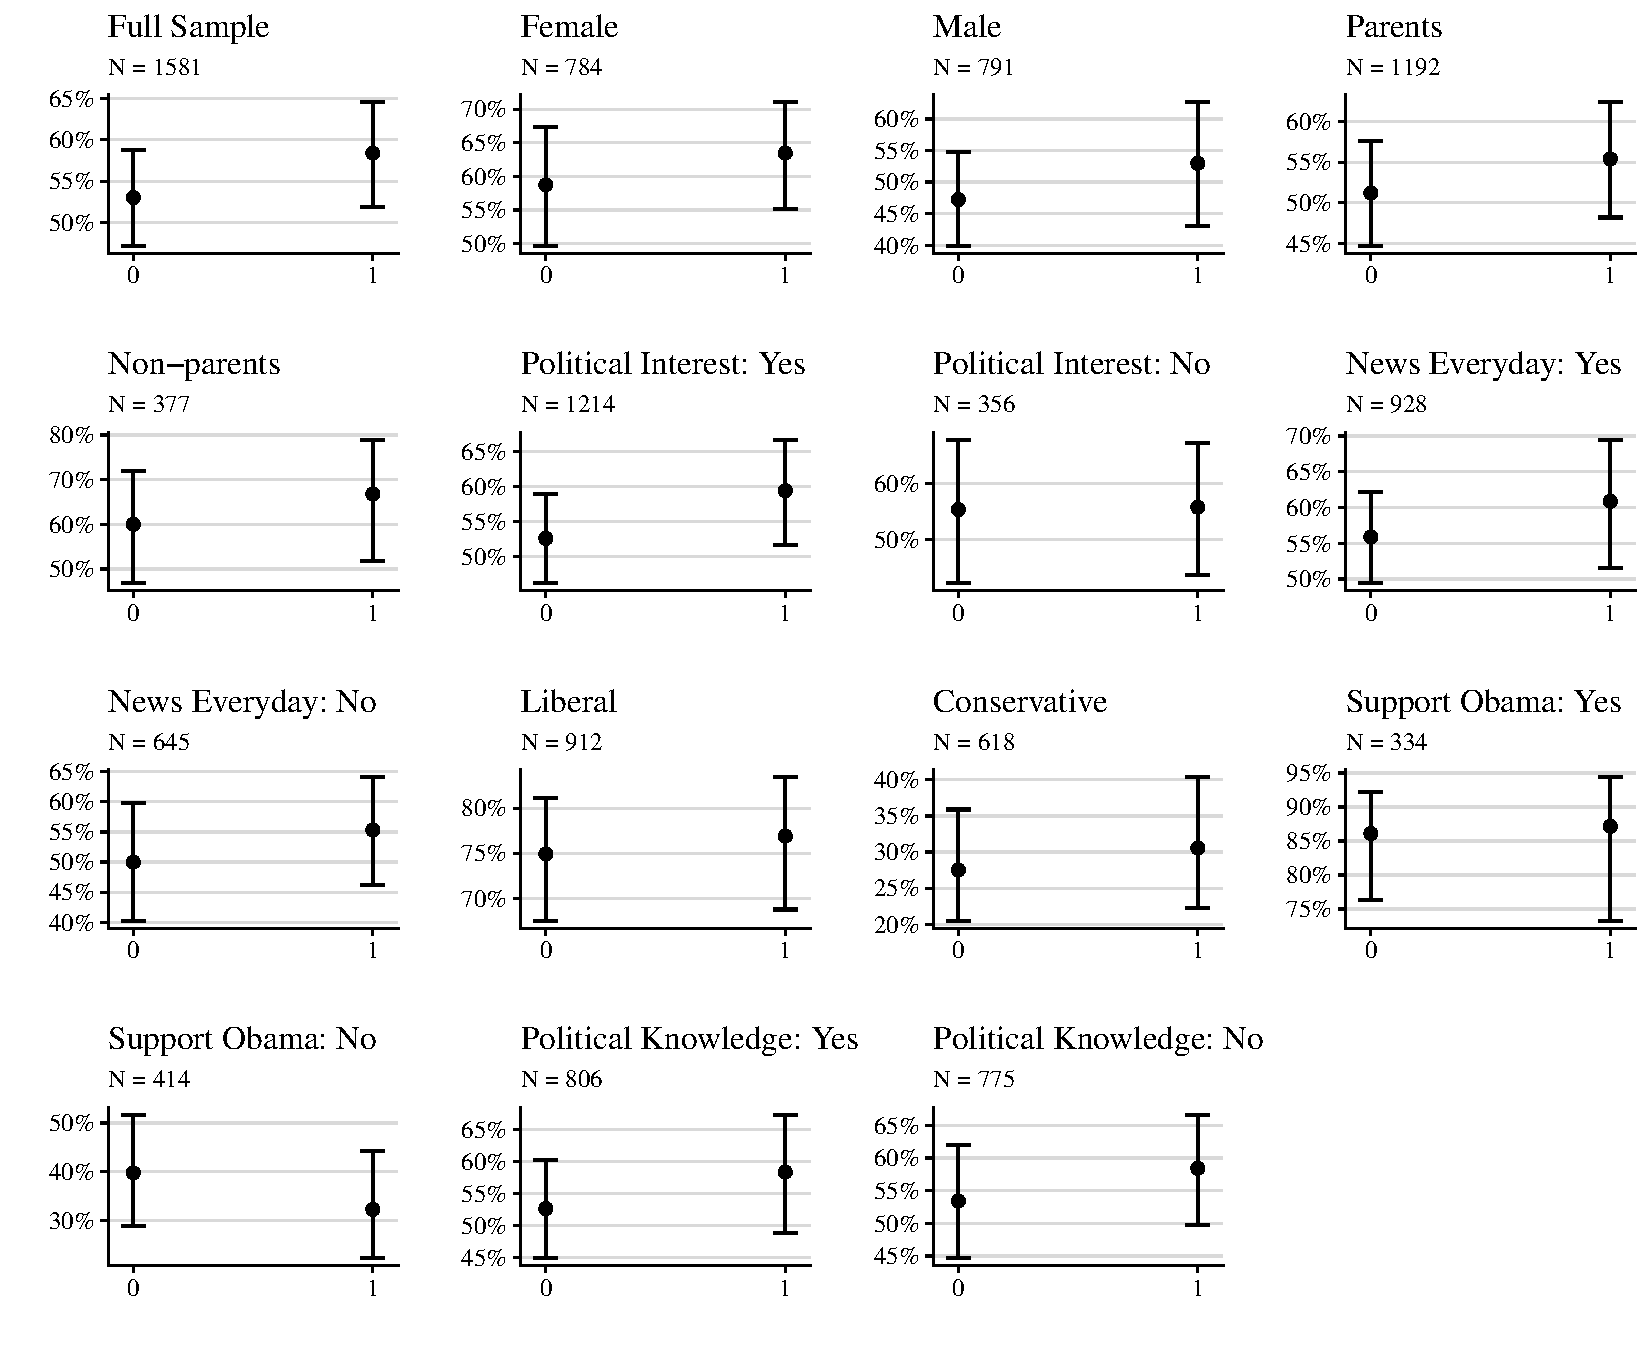
\includegraphics[width = 0.9\linewidth]{/Users/mz/Box/repository/replication/rogowski_tucker_2019_psrm/figs/fig2.pdf}
    \captionsetup{justification = raggedright, singlelinecheck = false}
    \caption{Predicted probabilities of gun control support before and after the 2016 Orlando shooting. In the \(x\)-axis, 0 means pre-shooting and 1 means post-shooting. The error bars show the 95\% confidence intervals, which are calculated by the Delta method. The survey weight is applied in the analysis.}
\end{figure}
\begin{figure}[htbp!]
    \centering
    \label{fig3}
    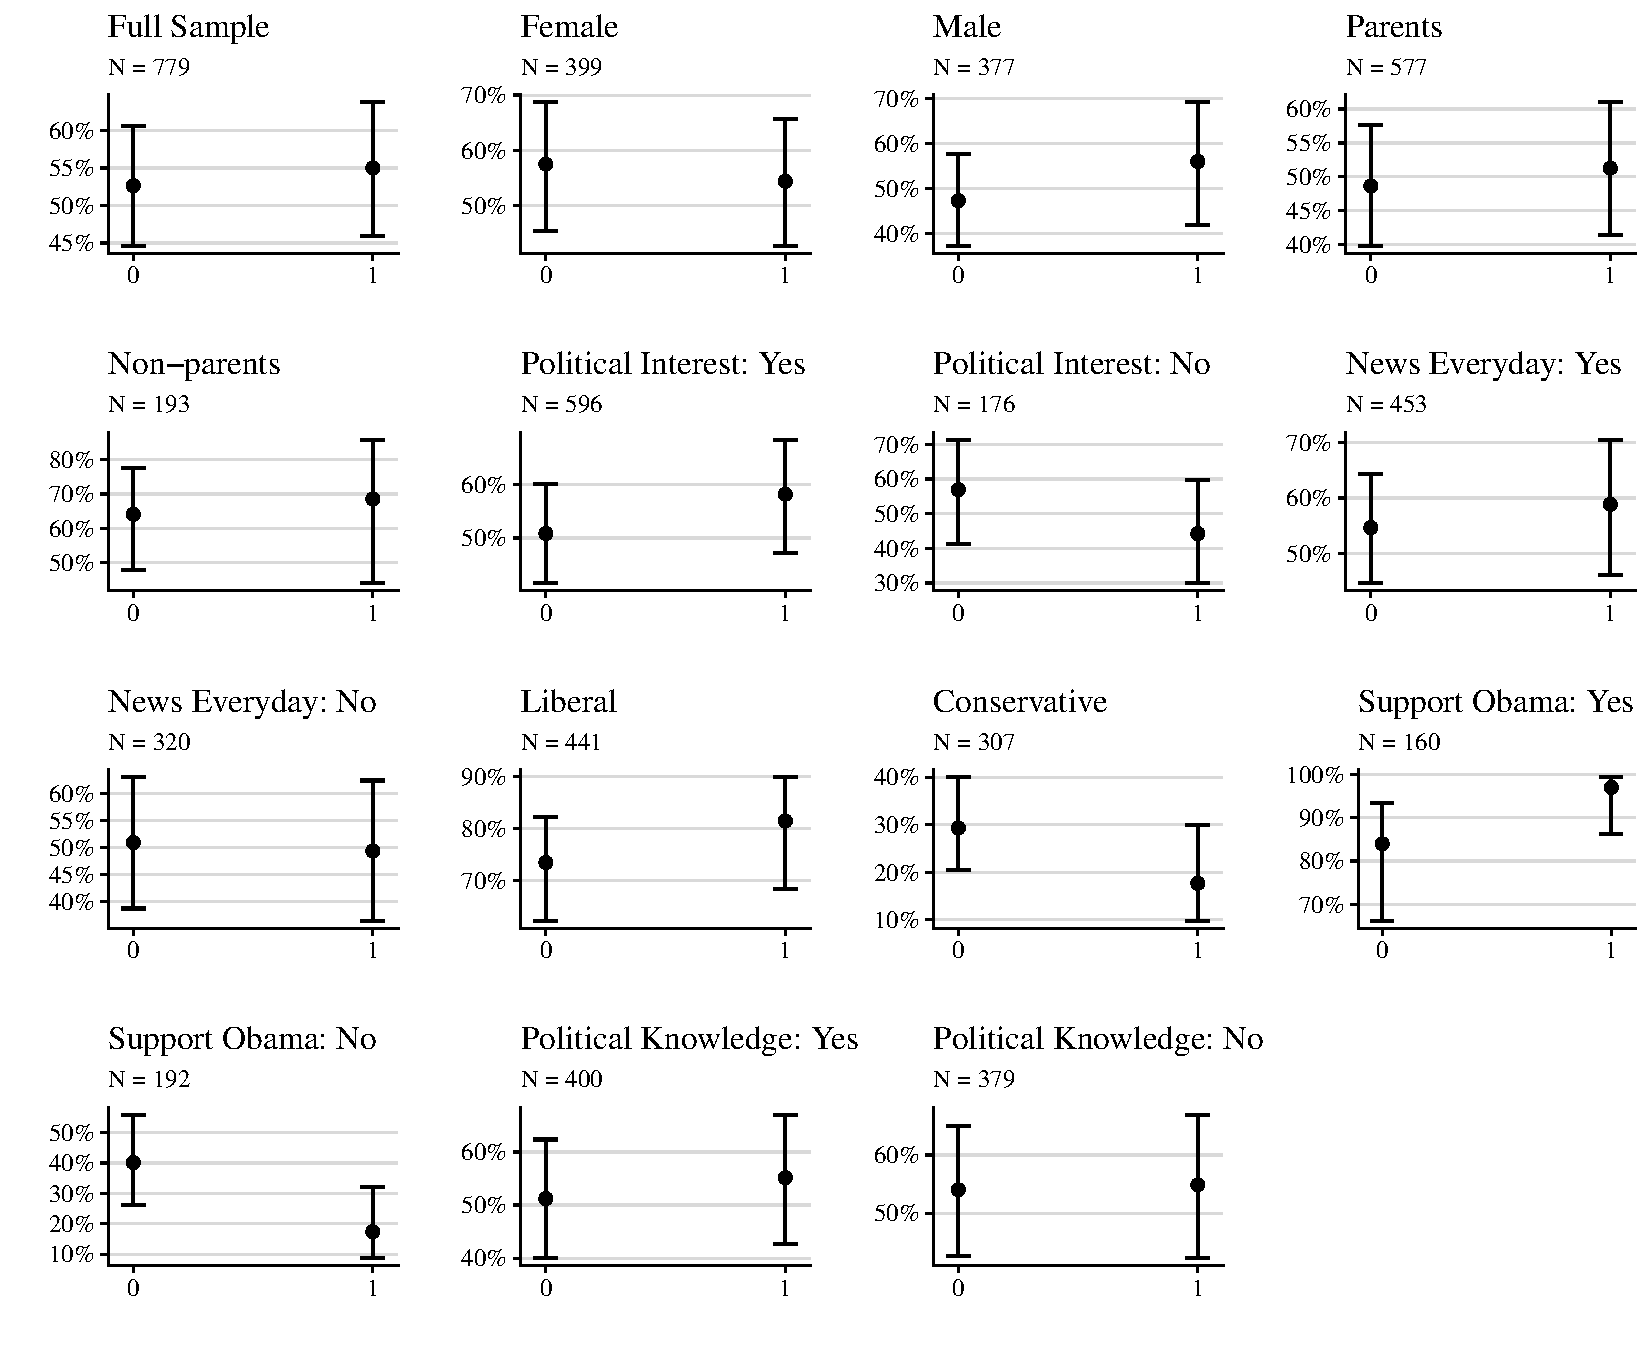
\includegraphics[width = 0.9\linewidth]{/Users/mz/Box/repository/replication/rogowski_tucker_2019_psrm/figs/fig3.pdf}
    \captionsetup{justification = raggedright, singlelinecheck = false}
    \caption{Predicted probabilities of gun control support before and after the 2016 Orlando shooting. The sample now only includes the respondents who finished the survey within 3 days before and 7 days after the shooting. In the \(x\)-axis, 0 means pre-shooting and 1 means post-shooting. The error bars show the 95\% confidence intervals, which are calculated by the Delta method. The survey weight is applied in the analysis.}
\end{figure}

\clearpage
\section*{Concluding Remarks}
\begin{itemize}
    \item By using alternative estimation frameworks, we show the null finding reported in RT is robust. That said, mass shooting does not change American people’s gun control support.
    \item We extend RT’s research by using the 2016 Orlando shooting. With a better-measured dependent variable, we still find the same result as that in RT.
    \item We argue non-compliance may drive the null finding. In future research employing a similar design, i.e., using the staggered survey completion to evaluate an exogenous event’s causal effect, scholars should consider more on this issue.
\end{itemize}

\newpage
\section*{References}
\begingroup
\setstretch{1.0}
\setlength\bibitemsep{0pt}
\printbibliography[heading = none]
\endgroup

\newpage
\section*{Appendix}
% latex table generated in R 4.0.0 by xtable 1.8-4 package
% Wed May 13 22:27:10 2020
\begin{table}[!htbp]
\centering
\caption{Effect of the Sandy Hook Shooting on Gun Control Support (Binary), Cross-sectional Analysis} 
\label{atab1}
\begin{tabular}{lrcrrr}
  \toprule
 & Estimate & Standard Error & \(t\)-statistic & \(p\)-value & \(N\) \\ 
  \midrule
Full Sample & $-$0.004 & 0.033 & $-$0.118 & 0.906 & 1684 \\ 
  Democrats & 0.003 & 0.060 & 0.046 & 0.963 & 645 \\ 
  Republicans & 0.010 & 0.039 & 0.269 & 0.788 & 438 \\ 
  Independents & $-$0.027 & 0.058 & $-$0.466 & 0.641 & 601 \\ 
  Liberal & 0.058 & 0.069 & 0.841 & 0.401 & 538 \\ 
  Moderate & $-$0.058 & 0.067 & $-$0.870 & 0.385 & 414 \\ 
  Conservative & $-$0.060 & 0.040 & $-$1.487 & 0.138 & 602 \\ 
  Female & 0.003 & 0.046 & 0.071 & 0.943 & 866 \\ 
  Male & $-$0.014 & 0.046 & $-$0.295 & 0.768 & 818 \\ 
  Parents & $-$0.085 & 0.054 & $-$1.583 & 0.114 & 454 \\ 
  Non-parents & 0.032 & 0.047 & 0.685 & 0.494 & 1038 \\ 
  NRA Membership: Yes & 0.164 & 0.186 & 0.882 & 0.379 & 118 \\ 
  NRA Membership: No & $-$0.022 & 0.034 & $-$0.650 & 0.516 & 1466 \\ 
  Proximity: Yes & $-$0.017 & 0.092 & $-$0.182 & 0.856 & 253 \\ 
  Proximity: No & $-$0.006 & 0.034 & $-$0.176 & 0.860 & 1431 \\ 
   \bottomrule
 \multicolumn{5}{l} {\footnotesize It replicates the numerical results underlying the left panel of Figure 2 in RT.}\\
 \multicolumn{5}{l} {\footnotesize Standard errors are heteroskedasticity-robust.}\end{tabular}
\end{table}

% latex table generated in R 4.0.0 by xtable 1.8-4 package
% Wed May 13 22:27:10 2020
\begin{table}[!htbp]
\centering
\caption{Effect of the Sandy Hook Shooting on Gun Control Support (Binary), Panel (First-difference) Analysis} 
\label{atab2}
\begin{tabular}{lrcrrr}
  \toprule
 & Estimate & Standard Error & \(t\)-statistic & \(p\)-value & \(N\) \\ 
  \midrule
Full Sample & $-$0.039 & 0.023 & $-$1.718 & 0.086 & 1066 \\ 
  Democrats & $-$0.051 & 0.041 & $-$1.257 & 0.210 & 394 \\ 
  Republicans & 0.032 & 0.029 & 1.097 & 0.274 & 289 \\ 
  Independents & $-$0.084 & 0.042 & $-$2.004 & 0.046 & 383 \\ 
  Liberal & $-$0.082 & 0.027 & $-$3.079 & 0.002 & 343 \\ 
  Moderate & 0.010 & 0.045 & 0.220 & 0.826 & 252 \\ 
  Conservative & $-$0.072 & 0.035 & $-$2.045 & 0.042 & 398 \\ 
  Female & $-$0.060 & 0.033 & $-$1.833 & 0.067 & 515 \\ 
  Male & $-$0.018 & 0.032 & $-$0.558 & 0.577 & 551 \\ 
  Parents & 0.011 & 0.051 & 0.216 & 0.829 & 259 \\ 
  Non-parents & $-$0.084 & 0.025 & $-$3.377 & 0.001 & 691 \\ 
  NRA Membership: Yes & $-$0.050 & 0.052 & $-$0.954 & 0.343 & 95 \\ 
  NRA Membership: No & $-$0.036 & 0.026 & $-$1.407 & 0.160 & 942 \\ 
  Proximity: Yes & $-$0.046 & 0.028 & $-$1.667 & 0.098 & 150 \\ 
  Proximity: No & $-$0.038 & 0.027 & $-$1.409 & 0.159 & 916 \\ 
   \bottomrule
 \multicolumn{5}{l}
 {\footnotesize It replicates the numerical results underlying the right panel of Figure 2 in RT.}\\
 \multicolumn{5}{l} {\footnotesize Standard errors are heteroskedasticity-robust.}\end{tabular}
\end{table}

% latex table generated in R 4.0.0 by xtable 1.8-4 package
% Wed May 13 22:27:10 2020
\begin{table}[!htbp]
\centering
\caption{Effect of the Sandy Hook Shooting on Gun Control Support (5-points Likert Scale), Cross-sectional Analysis} 
\label{atab3}
\begin{tabular}{lrcrrr}
  \toprule
 & Estimate & Standard Error & \(t\)-statistic & \(p\)-value & \(N\) \\ 
  \midrule
Full Sample & 0.052 & 0.105 & 0.499 & 0.618 & 1684 \\ 
  Democrats & $-$0.050 & 0.189 & $-$0.263 & 0.793 & 645 \\ 
  Republicans & 0.150 & 0.135 & 1.107 & 0.269 & 438 \\ 
  Independents & 0.041 & 0.180 & 0.227 & 0.820 & 601 \\ 
  Liberal & 0.021 & 0.216 & 0.096 & 0.924 & 538 \\ 
  Moderate & 0.029 & 0.206 & 0.143 & 0.887 & 414 \\ 
  Conservative & 0.040 & 0.158 & 0.256 & 0.798 & 602 \\ 
  Female & $-$0.034 & 0.146 & $-$0.231 & 0.817 & 866 \\ 
  Male & 0.141 & 0.153 & 0.918 & 0.359 & 818 \\ 
  Parents & $-$0.225 & 0.184 & $-$1.227 & 0.221 & 454 \\ 
  Non-parents & 0.113 & 0.147 & 0.767 & 0.443 & 1038 \\ 
  NRA Membership: Yes & 0.653 & 0.735 & 0.888 & 0.376 & 118 \\ 
  NRA Membership: No & $-$0.021 & 0.110 & $-$0.189 & 0.850 & 1466 \\ 
  Proximity: Yes & $-$0.024 & 0.293 & $-$0.081 & 0.935 & 253 \\ 
  Proximity: No & 0.056 & 0.111 & 0.510 & 0.610 & 1431 \\ 
   \bottomrule
 \multicolumn{5}{l}
 {\footnotesize It replicates the numerical results underlying the left panel of Figure A.1 in RT.}\\
 \multicolumn{5}{l} {\footnotesize Standard errors are heteroskedasticity-robust.}\end{tabular}
\end{table}

% latex table generated in R 4.0.0 by xtable 1.8-4 package
% Wed May 13 22:27:11 2020
\begin{table}[!htbp]
\centering
\caption{Effect of the Sandy Hook Shooting on Gun Control Support (5-points Likert Scale), Panel (First-difference) Analysis} 
\label{atab4}
\begin{tabular}{lrcrrr}
  \toprule
 & Estimate & Standard Error & \(t\)-statistic & \(p\)-value & \(N\) \\ 
  \midrule
Full Sample & $-$0.110 & 0.055 & $-$2.006 & 0.045 & 1066 \\ 
  Democrats & $-$0.113 & 0.073 & $-$1.565 & 0.118 & 394 \\ 
  Republicans & 0.028 & 0.074 & 0.377 & 0.706 & 289 \\ 
  Independents & $-$0.213 & 0.115 & $-$1.850 & 0.065 & 383 \\ 
  Liberal & $-$0.147 & 0.070 & $-$2.115 & 0.035 & 343 \\ 
  Moderate & $-$0.017 & 0.090 & $-$0.185 & 0.853 & 252 \\ 
  Conservative & $-$0.195 & 0.098 & $-$2.000 & 0.046 & 398 \\ 
  Female & $-$0.193 & 0.073 & $-$2.658 & 0.008 & 515 \\ 
  Male & $-$0.024 & 0.081 & $-$0.298 & 0.766 & 551 \\ 
  Parents & $-$0.012 & 0.099 & $-$0.123 & 0.902 & 259 \\ 
  Non-parents & $-$0.225 & 0.072 & $-$3.138 & 0.002 & 691 \\ 
  NRA Membership: Yes & $-$0.226 & 0.210 & $-$1.076 & 0.285 & 95 \\ 
  NRA Membership: No & $-$0.109 & 0.057 & $-$1.914 & 0.056 & 942 \\ 
  Proximity: Yes & $-$0.014 & 0.099 & $-$0.145 & 0.885 & 150 \\ 
  Proximity: No & $-$0.129 & 0.062 & $-$2.068 & 0.039 & 916 \\ 
   \bottomrule
 \multicolumn{5}{l}
 {\footnotesize It replicates the numerical results underlying the right panel of Figure A.1 in RT.}\\
 \multicolumn{5}{l} {\footnotesize Standard errors are heteroskedasticity-robust.}\end{tabular}
\end{table}

% latex table generated in R 4.0.0 by xtable 1.8-4 package
% Wed May 13 22:27:11 2020
\begin{table}[!htbp]
\centering
\caption{Effect of the Sandy Hook shooting on Gun Control Support Polarization} 
\label{atab5}
\begin{tabular}{lrcrrr}
  \toprule
 & Estimate & Standard Error & \(t\)-statistic & \(p\)-value & \(N\) \\ 
  \midrule
Supporters vs Opponents & $-$1.118 & 0.146 & $-$7.675 & 0.000 & 920 \\ 
  Democrats vs Republicans & $-$0.141 & 0.104 & $-$1.365 & 0.173 & 1065 \\ 
  Liberal vs Conservative & 0.048 & 0.120 & 0.400 & 0.689 & 1064 \\ 
   \bottomrule
 \multicolumn{5}{l}
 {\footnotesize It replicates the numerical results underlying Figure 3 in RT.}\\
 \multicolumn{5}{l}
 {\footnotesize We do not discuss this table in the main text. See RT for more details.}\end{tabular}
\end{table}


\begin{table}
\caption{Survey Completion Date and Gun Control Question No Opinion Rate}
\begin{center}
\begin{tabular}{l D{.}{.}{4.5}}
\toprule
 & \multicolumn{1}{c}{(Logit)} \\
\midrule
Post-shooting (Yes = 1) & -0.09      \\
                        & (0.20)     \\
Constant                & 2.65^{***} \\
                        & (0.14)     \\
\midrule
BIC                     & 800.77     \\
\(\ln\mathcal{L}\)      & -393.03    \\
\(N\)                   & 1568       \\
\bottomrule
\multicolumn{2}{l}{\scriptsize{Standard errors in parentheses. $^{***}p<0.001$; $^{**}p<0.01$; $^{*}p<0.05$.}}
\end{tabular}
\label{atab6}
\end{center}
\end{table}


\end{document}